%!TEX root=./main.tex
\section{Problem Statement and Overview of Results}

In this section we provide a formulation of the backpropagation
algorithm to establish notation and the context for our analysis. We then
formulate the feedback aligment algorithm that uses random backpropation weights.
A high-level overview of our results is then presented, together with
some of the intuition and proof techniques behind these results; we also contrast with what was known previously.

We mainly consider two-layer neural networks in the regression setting, specified by a family of functions  $f:\Rd \to \RR$ with input dimension $d$, sample size $n$, and $p$ neurons in the hidden layer. For an input $x\in\Rd$, the network outputs
\begin{align}\label{eqn:nonlinear-network}
    f(x) = \frac{1}{\sqrt p}\sum_{r=1}^p\beta_r\psi(w_r\transpose x)= \frac{1}{\sqrt p}\beta\transpose\psi(Wx),
\end{align}
where $W = (w_1,...,w_p)\transpose\in\Rpd$ and $\beta = (\beta_1,...,\beta_p)\transpose\in\Rp$ represent the feed-forward weights in the first and second layers, and $\psi$ denotes an element-wise activation function. The scaling by $\sqrt{p}$ is simply for convenience in the analysis.

Given $n$ input-response pairs $\{(x_i,y_i)\}_{i=1}^n$, the training objective is to minimize the mean squared error
\begin{equation}\label{eqn:squared-loss}
    \Loss(W,\beta) = \frac{1}{2n}\sum_{i=1}^n \big(y_i - f(x_i)\big)^2.
\end{equation}
Standard gradient descent attempts to minimize \eqref{eqn:nonlinear-network} by updating the feed-forward weights following gradient directions according to
\begin{align*}
    \beta_r(t+1) &= \beta_r(t)-\eta\frac{\partial\Loss}{\partial \beta_r}(W(t),\beta(t)) \quad\\ w_r(t+1) &= w_r(t)-\eta\frac{\partial\Loss}{\partial w_r}(W(t),\beta(t)),
\end{align*}
for each $r\in[p]$, where $\eta>0$ denotes the step size. We initialize $\beta(0)$ and $w_r(0)$  standard Gaussian vectors. We introduce the notation $f(t), e(t)\in \R^n$, with $f_i(t) = f(x_i)$ denoting the network output on input $x_i$ when the weights are $W(t)$ and $\beta(t)$, and $e_i(t) = y_i-f_i(t)$ denoting the corresponding prediction error or residual. With this notation,
the gradients are expressed as
\begin{equation*}
    \frac{\partial\Loss}{\partial \beta_r} = \frac{1}{\sqrt p}\sum_{i=1}^n e_i\psi(w_r\transpose x_i), \quad
    \frac{\partial\Loss}{\partial w_r} = \frac{1}{\sqrt p} \sum_{i=1}^n e_i \beta_r\psi'(w_r\transpose x_i)x_i.
\end{equation*}
Here it is seen that the the gradient of the first-layer weights $\frac{\partial \Loss}{\partial w_r}$ involves not only the local input $x_i$ and the change in
the response of the $r$-th neuron, but also the backpropagated error signal $e_i\beta_r$.
The appearance of $\beta_r$ is, of course, due to the chain rule; but in effect it requires that the forward weights between layers are identical to the backward weights under error propagation. There is no evidence of biological mechanisms that would enable such ``synaptic symmetry.''

\begin{figure*}[t]
  \begin{tabular}{cc}
    \hskip-10pt
    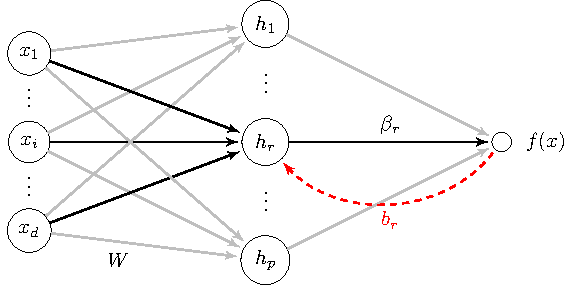
\includegraphics[width=.50\textwidth]{fig/fasketch}&\\[-1.6in]
    &
    \hskip-5pt
    \begin{minipage}{.47\textwidth}
    \begin{algorithm}[H]
    \centering
    \caption{Feedback Alignment}\label{algo:fa}
        \begin{algorithmic}[1]
            \Require Dataset $\{(x_i,y_i)\}_{i=1}^n$, step size $\eta$
            \State {\bf initialize} $W$, $\beta$ and $b$ as Gaussian
            \While{not converged}
                \State $\beta_r \gets \beta_r - \frac{\eta}{\sqrt p} \sum_{i=1}^n e_i \psi(w_r\transpose x_i)$
                \State $w_r \gets w_r - \frac{\eta}{\sqrt{p}} \sum_{i=1}^n e_i b_r\psi'(w_r\transpose x_i)x_i$
                \State for $r\in[p]$
            \EndWhile
        \end{algorithmic}
    \end{algorithm}%
    \end{minipage}
    \\[1.05in]

  \end{tabular}
\caption{Standard backpropagation updates the first layer weights for a hidden node $r$ with the second layer feedforward weight $\beta_r$. We study the procedure where the error is backpropagated instead using a fixed, random weight $b_r$.}
\label{fig:algo}
\end{figure*}


In the \textit{feedback alignment} procedure of \citep{lillicrap2016random},
when updating the weights $w_r$, the error signal is weighted, and propagated backward, not by the second layer feedforward weights $\beta$, but rather by a random set of weights $b\in\reals^p$ that are fixed during the course of training. Equivalently, the gradients for the first layer are
replaced by the terms
\begin{align}\label{eqn:alignment-update}
  \widetilde{\frac{\partial\Loss}{\partial w_r}}   = \frac{1}{\sqrt{p}} \sum_{i=1}^n e_i b_r\psi'(w_r\transpose x_i)x_i.
\end{align}
Note, however, that this update rule does not correspond to the gradient with
respect to a modified loss function. The use of a random weight $b_r$ when updating
the first layer weights $w_r$ does not violate locality, and could conceivably be implemented by biological mechanisms; we refer to \cite{lillicrap2016random,bartunov,lillicrap2020backpropagation} for further discussion. A schematic of the relationship between the two algorithms is shown in Figure~\ref{fig:algo}.

We can now summarize the main results and contributions of this paper. Our first result shows that the error converges to zero when using random backpropagation weights.

\begin{itemize}
  \item Under Gaussian initialization of the parameters, if the model is sufficiently over-parameterized with $p\gg n$, then the error converges to zero linearly. Moreover, the parameters satisfy $\|w_r(t) - w_0(t) \| = \widetilde O\bigl(\frac{n}{\sqrt{p}}\bigr)$
    and $|\beta_r(t) - \beta_0(t) | = \widetilde O\bigl(\frac{n}{\sqrt{p}}\bigr)$.
\end{itemize}
The precise assumptions and statement of this result are given in \cref{thm:nonliner_conv}. The proof
shows that in the over-parameterized regime that the weights only change
by a small amount. While related to results for standard gradient descent,
new methods are required because the ``effective kernel'' is not positive semi-definite.

We next turn to the issue of alignment of the second layer parameters $\beta$ with the random backpropagation weights $b$. Such alignment was first observed in the original simulations of \cite{lillicrap2016random}. With $h\in \R^p$ denoting the hidden layer of the two-layer network,  the term $\dbp(h) \defeq \frac{\partial \Loss}{\partial h}$ represents
how the error signals are sent backward to update the feed-forward weights.
It is easy to calculate that
$\dbp(h) = \beta \sum_{i=1}^n e_i$ for error terms $e_i$. With the use of random backpropagation weights, the error is instead propagated backward as $\dfa(h) = b \sum_{i=1}^n e_i$.


\citet{lillicrap2016random} notice a decreasing angle between $\dbp(h)$ and $\dfa(h)$ during training, which is a sufficient condition to ensure that the algorithm converges.
In the case of $k$-way classification, the last layer has $k$ nodes,
$\beta$ and $b$ are $p\times k$ matrices, and each error term $e_i$ is a $k$-vector.
In the regression setting that we focus on $k=1$, so that the angle between
$\dbp(h)$ and $\dfa(h)$ is the same as the angle between $\beta$ and $b$.
Intuitively, the possibility for alignment is seen in the fact that while the updates for $W$ use the error weighted by the random weights $b$, the updates for $\beta$ indirectly involve $W$, allowing for the possibility that dependence on $b$ will be introduced into $\beta$.

Our first result shows that, in fact, alignment will \textit{not} occur in the over-parameterized setting. (So, while the error may still converge, ``feedback alignment'' may be a bit of a misnomer for the algorithm.)
\begin{itemize}
\item The cosine of the angle between
the $p$-dimensional vectors $\dfa$ and $\dbp$ satisfies $
\cos\angle(\dfa, \dbp(t)) = \cos\angle(b, \beta(t)) = O\big(\frac{n}{\sqrt p}\big)$.

\end{itemize}
 However, we show that regularizing the parameters will cause
 $\dbp$ to align with $\dfa$ and therefore the parameters $\beta$ to align with $b$. Since $\beta(0)$ and $b$ are high dimensional Gaussian vectors, they are nearly orthogonal with high probability. The effect of regularization can be seen as shrinking the component of $\beta(0)$ in the parameters over time.  Our next result establishes this precisely in the linear case.
\begin{itemize}
\item Supposing that $\psi(u)=u$, then introducing a ridge penalty $\lambda(t) \|\beta\|^2$ where $\lambda(t) = \lambda$ for $t\leq T$ and $\lambda(t) = 0$ for $t > T$
on $\beta$  causes the parameters to align, with $\cos\angle(b, \beta(t)) \geq c > 0$ for sufficiently large $t$.
\end{itemize}
The technical conditions are given in \cref{thm:lin_align}.
Our simulations are consistent with this result, and also show alignment with a constant regularization $\lambda(t)\equiv \lambda$, for both linear and nonlinear activation functions. Finally, we complement this result by showing that convergence is preserved with regularization, for general activation functions. This is presented in \cref{thm:nonlinear_conv_reg}.
